\documentclass[12pt,fleqn]{fancybook} % Default font size and left-justified eqns
\usepackage[noTeX]{mmap}
\usepackage{mycommands} % put first or some of our custom packages may break formatting.
%%% This file is generated by Makefile.
%%% Do not edit this file!
%%%
	\gdef\GITAbrHash{0562524}	\gdef\GITAuthorDate{Wed May 21 10:46:42 2014 -0400}	\gdef\GITAuthorName{Nate Iverson}
\usepackage{makeidx}
\makeindex
\author{Nathaniel Iverson%
\and
S\"{o}nmez \c{S}ahuto\u{g}lu}
\title{INTRODUCTION TO LINEAR ALGEBRA}
\date{2014}


\makeindex

\begin{document}
\frontmatter

\maketitle

\begin{copyrightpage}
\noindent Licensed under the Creative Commons Attribution-NonCommercial 3.0 Unported License (the ``License''). You may not use this file except in compliance with the License. You may obtain a copy of the License at \url{http://creativecommons.org/licenses/by-nc/3.0}. Unless required by applicable law or agreed to in writing, software distributed under the License is distributed on an \textsc{``as is'' basis, without warranties or conditions of any kind}, either express or implied. See the License for the specific language governing permissions and limitations under the License.\\ % License information
\end{copyrightpage}

\chapterimage{Pictures/chapter_head_1.pdf}
\tableofcontents

\mainmatter

\chapterimage{chapter_head_2.pdf} % Chapter heading image
\chapter{$\mathbb{R}^n$ and Real Matrices}
\index{$\mathbb{R}^n$}\index{Matrix}
\section{Introduction}
\index{$\mathbb{R}^n$, Introduction}
\subsection{$\mathbb{R}^n$}
We will assume that all readers are already familiar with a concept of real and complex numbers. In this text we denote the real numbers by $\mathbb{R}$ and the complex numbers by $\mathbb{C}$. 

\begin{definition}
We define $\mathbb{R}^n$ to be the set of real column vectors in $n$-coordinates. That is 
\[
\mathbb{R}^n=\left\{ 
\begin{bmatrix}
x_1\\ x_2 \\ \vdots \\ x_n
\end{bmatrix} 
: x_i \in \mathbb{R}\text{ for all }i=1,2, \ldots, n \right\}
\]

We will refer to the members of $\mathbb{R}^n$ as \emph{vectors} and the 
elements of $\mathbb{R}$ as \emph{scalars}. When we want to refer to row vectors 
instead of column vectors we will use the notation $\mathbb{R}^n_\text{row}$.
\end{definition}

For convenience we may refer to each $\vec{x} \in \mathbb{R}^n$ as a single 
bold letter where we will for allow each coordinate be labeled as the same 
subscriped letter. For example
\[
\vec{x}=\begin{bmatrix}x_1\\ x_2 \\ \vdots \\ x_n\end{bmatrix}
\vec{y}=\begin{bmatrix}y_1\\ y_2 \\ \vdots \\ y_n\end{bmatrix}
\vec{v}=\begin{bmatrix}v_1\\ v_2 \\ \vdots \\ v_n\end{bmatrix}
\]

\begin{remark}
Sometimes it is useful to describe a vector as a function on it's coordinates. 
For example if 
$\vec{v}=\begin{bmatrix}1 \\ 4 \\ 9 \end{bmatrix}$ We may say 
$\vec{v}(2)=4$ that is the 2nd coordinate of $\vec{v}$ is $4$.
\end{remark}


\begin{definition}\index{vector equality}
Vectors $\vec{v}, \vec{w} \in \mathbb{R}^n$ are \emph{equal},  if they are equal 
coordinatewise. That is, $v_i=v(i)=w(i)=w_i$ for all $i=1,2,\ldots, n$. We 
denote this with  $\vec{v}=\vec{w}$.
\end{definition}


\begin{definition}\index{vector addition}
We define \emph{vector addition} on $\mathbb{R}^n$ coordinatewise. That is for 
$\vec{v},\vec{w} \in \mathbb{R}^n$ we define
\[
\vec{v}+\vec{w}=
\begin{bmatrix}v_1\\ v_2 \\ \vdots \\ v_n\end{bmatrix}+
\begin{bmatrix}w_1\\ w_2 \\ \vdots \\ w_n\end{bmatrix}=
\begin{bmatrix}v_1+w_1\\ v_2+w_2 \\ \vdots \\ v_n+w_n\end{bmatrix}
\]
\end{definition}

\begin{definition}]\index{scalar multiplication}
We define \emph{scalar multiplication} on $\mathbb{R}^n$ coordinatewise. That 
is for $\vec{v} \in \mathbb{R}^n$ and $r \in \mathbb{R}$ we define
\[
r\vec{v}=
r\begin{bmatrix}v_1\\ v_2 \\ \vdots \\ v_n\end{bmatrix}=
\begin{bmatrix}rv_1\\ rv_2 \\ \vdots \\ rv_n\end{bmatrix}
\]
\end{definition}

The order of operations is scalar multiplication first then vector addition.

\begin{example}
Consider  $\vec{x}=\begin{bmatrix*}[r]1\\ 0  \\ -3\end{bmatrix*}$ and 
$\vec{y}=\begin{bmatrix*}[r]-4\\ 2 \\ 1\end{bmatrix*}$ in $\mathbb{R}^3$.
\[
2\vec{x}+(-1)\vec{y}=
2\begin{bmatrix*}[r]1\\ 0  \\ -3\end{bmatrix*}+
(-1)\begin{bmatrix*}[r]-4\\ 2 \\ 1\end{bmatrix*}=
%\begin{bmatrix}2(1)\\ 2(0)  \\ 2(-3)\end{bmatrix}+
%\begin{bmatrix}(-1)(-4)\\ (-1)(2) \\ (-1)(1)\end{bmatrix}=
\begin{bmatrix*}[r]2\\ 0  \\ -6\end{bmatrix*}+
\begin{bmatrix*}[r]4\\ -2 \\ -1\end{bmatrix*}=
\begin{bmatrix}2+4\\ 0+(-2)  \\ -6+(-1)\end{bmatrix}=
\begin{bmatrix*}[r]6\\ -2  \\ -5\end{bmatrix*}
\]
This is actually also an example of our next definition.
\end{example}
\begin{definition}\index{linear combination}
A \emph{linear combination} of vectors $\vec{a}_1, \vec{a}_2, \ldots, 
\vec{a}_n$ is the sum  
\[c_1\vec{a}_1+c_2\vec{a}+\cdots+c_n\vec{a}_n\]  
for some choice of scalar multiples $c_1,c_2, \ldots, c_n \in \mathbb{R}$
\end{definition}


\begin{example}
Any vector in $\mathbb{R}^2$ can be written as a linear combination of 
$\begin{bmatrix}1 \\ 0\end{bmatrix}$ and $\begin{bmatrix}1 \\ 1 \end{bmatrix}$ 
because 
\[
\begin{bmatrix}v_1 \\ v_2\end{bmatrix}=
(v_1-v_2) \begin{bmatrix}1 \\ 0\end{bmatrix}+
v_2 \begin{bmatrix}1 \\ 1 \end{bmatrix}
\]
\end{example}

\begin{example}
The vector $\begin{bmatrix}1 \\ 1\end{bmatrix}$ is not a linear combination 
of $\begin{bmatrix}1 \\ 0\end{bmatrix}$ and $\begin{bmatrix}2 \\ 
0\end{bmatrix}$. If it were then, we would have 
\[
\begin{bmatrix}1 \\ 1\end{bmatrix}=
a \begin{bmatrix}1 \\ 0\end{bmatrix}+
b \begin{bmatrix}2 \\ 0 \end{bmatrix}
\]
for some constants $a,b\in \mathbb{R}$. Considering the second components, this 
implies that $1=0$ which is a contradiction.
\end{example}

\begin{definition}
\index{standard basis for $\mathbb{R}^n$}
The \emph{standard basis for} $\mathbb{R}^n$ is a set of $n$-vectors 
$\{\vec{e}_1, \vec{e}_2, \ldots, \vec{e}_n\}$ such that
$\vec{e}_j(k)=\begin{cases}
1 & \text{ if } k=j\\
0 & \text{ if } k\neq j
\end{cases}$ 
for each $j,k \in \{1, 2, \ldots, n\}$
\end{definition}

\begin{example}
In $\mathbb{R}^3 $ every vector is a linear combination of the standard basis 
$\{\vec{e}_1,\vec{e}_2,\vec{e}_3\}$
\[
\begin{bmatrix}v_1 \\ v_2 \\ v_3\end{bmatrix}=
v_1 \begin{bmatrix}1 \\ 0 \\ 0\end{bmatrix}+
v_2 \begin{bmatrix}0 \\ 1 \\ 0\end{bmatrix}+
v_3 \begin{bmatrix}0 \\ 0 \\ 1\end{bmatrix}
=v_1\vec{e}_1+v_3\vec{e}_3+v_3\vec{e}_3
\]
\end{example}

\begin{proposition}
In $\mathbb{R}^n$ every vector is a linear combination of the standard basis 
$\{\vec{e}_1, \vec{e}_2, \ldots, \vec{e}_n\}$.
\end{proposition}

\begin{proof}
Let $\vec{v} \in \mathbb{R}^n$ and $1\leq k\leq n$. Then we observe that  
\[\vec{v}(k)=v_k=v_k\cdot 1=v_k \vec{e}_k(k).\]
We can rewrite this equation by adding $k-1$ zeros before and $n-k$ zeros 
after $\vec{v}(k)$. That is,  
\[\vec{v}(k)=0+ \cdots + 0+v_k\vec{e}_k(k)+0+\cdots+0.\] 
Since $\vec{e}_j(k)=0$ for all $j\neq k$ we have 
\[\vec{v}(k)=v_1\vec{e}_1(k)+v_2\vec{e}_2(k)+\cdots+ v_k\vec{e}_k(k)+ \cdots + 
v_n\vec{e}_n(k).\]
Since the above equation is true for any $1\leq k\leq n$ we have,  
\[\vec{v}=v_1\vec{e}_1+v_2\vec{e}_2+\cdots+ v_n\vec{e}_n.\]
\end{proof}


\subsection{Real Matrices}
\index{Real Matrices}

\begin{definition}
A real matrix $A$ is a rectangular array of real numbers $a_{i,j} \in 
\mathbb{R}$ (usually the comma is omitted $a_{ij}$)  where the $i$ is the row 
and $j$ is the column number. That is:
\[
A=[a_{ij}]=[\vec{a}_1, \vec{a}_2, \ldots, \vec{a}_n]=
\begin{bmatrix}
a_{11} & a_{12} & \cdots & a_{1n} \\
a_{21} & a_{22} & \cdots & a_{2n} \\
\vdots & \vdots & \ddots & \vdots \\
a_{m1} & a_{m2} & \cdots & a_{mn} 
\end{bmatrix}
\]
The \emph{dimension} of the matrix are $m\times n$ where $m$ is the number of 
rows and $n$ is the number of columns. 
\end{definition}
The matrix $A$ can be also seen as a collection of vectors. Namely, 
$A=[a_{ij}]=[\vec{a}_1, \vec{a}_2, \ldots, \vec{a}_n]$ where 
 $\vec{a}_1, \vec{a}_2,\ldots, \vec{a}_n \in \mathbb{R}^n$ are the \emph{column 
vectors} of $A$. In particular, 
\[
\vec{a}_1=\begin{bmatrix}a_{11}\\a_{21}\\ \vdots \\ a_{m1}\end{bmatrix}, \quad 
\vec{a}_2=\begin{bmatrix}a_{12}\\a_{22}\\ \vdots \\ a_{m2}\end{bmatrix}, 
\cdots, \quad 
\vec{a}_k=\begin{bmatrix}a_{1k}\\a_{2k}\\ \vdots \\ a_{mk}\end{bmatrix}, 
\cdots, \quad 
\vec{a}_n=\begin{bmatrix}a_{1n}\\a_{2n}\\ \vdots \\ a_{mn}\end{bmatrix}
\]

\begin{example}
$A=\begin{bmatrix*}[r]
2 & -3 & 0 \\
-5 & 0 & 1 
\end{bmatrix*}$
is a $2 \times 3$ matrix, $a_{12}=-3$, and  
$\vec{a}_1=\begin{bmatrix*}[r] 2 \\ -5 \end{bmatrix*} $
\end{example}

\subsection{Matrix-Vector Multiplication}

\begin{definition}\index{Matrix-Vector Multiplication}
Given an $m \times n$ matrix $A=[\vec{a}_1, \vec{a}_2, \ldots, \vec{a}_n]$ and 
column vector $\vec{v} \in \mathbb{R}^n$. We define the \emph{Matrix-Vector} 
product to be the linear combination 
\[
A\vec{v}=[\vec{a}_1, \vec{a}_2, \ldots ,\vec{a}_n]\begin{bmatrix}v_1 \\ v_2 \\ 
\vdots \\ v_n \end{bmatrix}=v_1\vec{a}_1+v_2\vec{a}_2+\cdots+v_n\vec{a}_n
\]
\end{definition} 
\begin{remark}
It is important to note that the product is only defined if the number of columns in $A$ matches the number of coordinates in $\vec{v}$.
\end{remark}

\begin{example}
\begin{align*}
\begin{bmatrix*}[r]
2 & -3 & 0 \\
-5 & 0 & 1 
\end{bmatrix*} 
\begin{bmatrix}1\\ 2 \\ 3 \end{bmatrix}
&=1\begin{bmatrix*}[r]2\\-5\end{bmatrix*} 
+2\begin{bmatrix*}[r]-3\\0\end{bmatrix*} 
+3\begin{bmatrix}0\\1\end{bmatrix}\\
&=\begin{bmatrix*}[r]2\\-5\end{bmatrix*}
+\begin{bmatrix*}[r]-6\\0\end{bmatrix*}+\begin{bmatrix}0\\3\end{bmatrix}\\
&=\begin{bmatrix*}[r]-4\\-2\end{bmatrix*}
\end{align*}
\end{example}

\begin{example}
\begin{align*}
\begin{bmatrix*}[r]
2 & -3 & 0 \\
-5 & 0 & 1 
\end{bmatrix*}
\begin{bmatrix}v_1\\ v_2 \\ v_3 \end{bmatrix}
&=v_1\begin{bmatrix*}[r]2\\-5 \end{bmatrix*}
+v_2\begin{bmatrix*}[r]-3 \\0\end{bmatrix*}
+v_3\begin{bmatrix}0\\1\end{bmatrix}\\
&=\begin{bmatrix*}[r]2v_1\\-5v_1\end{bmatrix*}
+\begin{bmatrix}-3v_2\\ 0\end{bmatrix} 
+\begin{bmatrix}0\\v_3\end{bmatrix}\\
&=\begin{bmatrix}2v_1-3v_2\\-5v_1+v_3\end{bmatrix}
\end{align*}
\end{example}


\section{Linear Transformations in $\mathbb{R}^n$}
\index{Linear Transformations}
\subsection{Definition}

\begin{definition}[Function]
A function $f:A \to B$ is a map the associates each value $a$ in the  
\emph{domain} $A$ with exactly one value $b$ in the \emph{codomain} $B$. 
We would write $f(a)=b$. We will call all the elements in $B$ actually mapped 
to by $f$ the \emph{image} of $A$ under $f$ and denote it 
$f(A)=\{ f(a):\text{ for } a \in A  \}$.
\end{definition}
\begin{example}$f:\mathbb{R} \to \mathbb{R}$ defined by $f(x)=x^2$ is a 
function. The domain  and the codomain are both $\mathbb{R}$ while the 
image is $f(\mathbb{R})=[0,\infty )$.
\end{example}
\begin{remark}
We are intentionally avoiding the term \emph{range} of a function because it is 
ambiguous. Some authors call the range the image and others call it the 
codomain.
\end{remark}
\begin{definition}[Linear Transformation]
A real \emph{linear transformation} is a function\\ 
$T: \mathbb{R}^n \to \mathbb{R}^m$ such that vector addition and scalar 
multiplication are preserved. That is, 
\begin{enumerate}
\item $T(\vec{v}+\vec{w})=T(\vec{v})+T(\vec{w})$ for all 
$\vec{v},\vec{w} \in \mathbb{R}^n$\hfill \emph{(preserves vector addition)}
\item $T(r\vec{v})=r T(\vec{v})$ for all $\vec{v}\in \mathbb{R}^n$ 
and for $r \in \mathbb{R}$\hfill \emph{(preserves scalar multiplication)}
\end{enumerate}
\end{definition}

\begin{proposition} If $A \in M_{m \times n}(\mathbb{R})$ then the function 
$T:\mathbb{R}^n \to \mathbb{R}^m$ defined by $T(\vec{v})=A\vec{v}$ is a linear 
transformation. This map is commonly referred to as $\vec{v} \to A\vec{v}$.
\label{prop:Av_is_linear}
\end{proposition}
\begin{proof}
Let $\vec{v},\vec{w} \in \mathbb{R}^n$ and $r \in \mathbb{R}$. 
We will start with scalar multiplication 
\begin{align*}
T(r\vec{v})
%=A\begin{bmatrix}av_1\\ \vdots \\ av_n\end{bmatrix}
&=[\vec{a}_1, \ldots, \vec{a}_n]
\begin{bmatrix}rv_1\\ \vdots \\  rv_n\end{bmatrix}\\
&=(r v_1)\vec{a}_1+\cdots+(r v_n)\vec{a}_n\\
&=r (v_1\vec{a}_1+\cdots+v_n\vec{a}_n)\\
&=r (A\vec{v})\\
&=r T(\vec{v})
\end{align*}
Now we show vector addition is preserved:
\begin{align*}
T(\vec{v}+\vec{w})
%&=A\begin{bmatrix}v_1+w_1\\ \vdots \\ v_n+w_n\end{bmatrix}\\
&=[\vec{a}_1, \ldots, \vec{a}_n]\begin{bmatrix}v_1+w_1\\ \vdots \\ v_n+w_n\end{bmatrix}\\
&=(v_1+w_1)\vec{a}_1+\cdots+(v_n+w_n)\vec{a}_n\\
&=(v_1\vec{a}_1+\cdots+v_n\vec{a}_n)+(w_1\vec{a}_1+\cdots+w_n\vec{a}_n)\\
&=A\vec{v}+A\vec{w}\\
&=T(\vec{v})+T(\vec{w})
\end{align*}
Note that the vector associative and distributive properties used above 
follow from the associative and distributive properties in $\mathbb{R}$ 
by applying them on each coordinate.

Since the choices of $\vec{v},\vec{w}$ and $r$ were arbitrary the proof 
works for all $\vec{v},\vec{w} \in \mathbb{R}^n$ and $r \in \mathbb{R}$.
\end{proof}

\begin{example} We will show that  map $T:\mathbb{R}^2 \to \mathbb{R}^3$ 
defined by 
$T\begin{bmatrix}v_1 \\ v_2 \end{bmatrix}=
\begin{bmatrix}v_1-3v_2\\v_2\\5v_1-3v_2\end{bmatrix}$
is a linear transformation.

Let $\vec{v},\vec{w} \in \mathbb{R}^n$. Then 
\begin{align*}
T(\vec{v}+\vec{w}) 
&= T\begin{bmatrix}v_1+w_1\\v_2+w_2\\v_3+w_3\end{bmatrix}\\
&= \begin{bmatrix}(v_1+w_1)-3(v_2+w_2)\\v_2+w_2\\5(v_1+w_1)-3(v_2+w_2)\end{bmatrix}\\
&= \begin{bmatrix}v_1-3v_2+w_1-3w_2\\v_2+w_2\\5v_1-3v_2+5w_1-3w_2\end{bmatrix}\\
&= \begin{bmatrix}v_1-3v_2\\v_2\\5v_1-3v_2\end{bmatrix}
+\begin{bmatrix}w_1-3w_2\\w_2\\5w_1-3w_2\end{bmatrix}\\
&= T(\vec{v})+T(\vec{w})
\end{align*}
Thus $T$ preserves addition. Let $r\in \mathbb{R}$ then 
\begin{align*}
T(r\vec{v}) 
&= T\begin{bmatrix}rv_1\\rv_2\\rv_3\end{bmatrix}\\
&= \begin{bmatrix}rv_1-3rv_2\\rv_2\\5rv_1-3rv_2\end{bmatrix}\\
&= \begin{bmatrix}r(v_1-3v_2)\\r(v_2)\\r(5v_1-3v_2)\end{bmatrix}\\
&= r\begin{bmatrix}v_1-3v_2\\v_2\\5v_1-3v_2\end{bmatrix}\\
&= rT(\vec{v})
\end{align*}
Thus $T$ is preserves scalar multiplication and is therefore a linear
transformation.
\end{example}

\begin{remark}
Notice that we write $T\begin{bmatrix}v_1\\v_2\\v_3\end{bmatrix}$ instead 
of  $T\left(\begin{bmatrix}v_1\\v_2\\v_3\end{bmatrix}\right)$ as a simple 
mater of convenience.
\end{remark}
\begin{proposition}
A linear transformation $T:\mathbb{R}^n \to \mathbb{R}^m$ has the property 1
that $T(\vec{0}_n)=\vec{0}_m$ where $\vec{0}_n \in \mathbb{R}^n$ and 
$\vec{0}_m \in \mathbb{R}$ are the zero vectors.
\end{proposition}

Proof of the above proposition is an exercise.

\begin{example}The map $T:\mathbb{R}^3 \to \mathbb{R}^2$ defined by 
$T\begin{bmatrix}v_1 \\ v_2 \\ v_3\end{bmatrix}=\begin{bmatrix}-7v_1+v_2 \\ 
v_1+v_2+3\end{bmatrix}$ 
is not a linear transformation because $T(\vec{0})=\begin{bmatrix}0\\3\end{bmatrix}$.
\end{example}

\begin{theorem}
Let $T:\mathbb{R}^n\to\mathbb{R}^m$ be a function. The following are equivalent:
\begin{enumerate}
\item $T$ is a linear transformation.
\item $T(a\vec{v}+b\vec{w})=aT(\vec{v})+bT(\vec{w})$ for all $a,b \in \mathbb{R}$ 
and $\vec{v},\vec{w} \in \mathbb{R}^n$
\item $T$ preserves linear transformations. That is, 
\[T(a_1\vec{v}_1+a_2\vec{v}_2+\cdots+a_k\vec{v}_k)=
a_1T(\vec{v}_1)+a_2T(\vec{v}_2)+\cdots+a_kT(\vec{v}_k)\] 
for all $a_i \in \mathbb{R}$ and $\vec{v}_i \in \mathbb{R}^n$ and $k$ a positive integer.
\end{enumerate}
\end{theorem}

\begin{proof}
We will show the equlivalence of all three by showing $1 \implies 2$ and 
$2 \implies 3$ and $3 \implies 1$. 
Then the rest of the implications can be deduced working around the circle:\\
\begin{center}
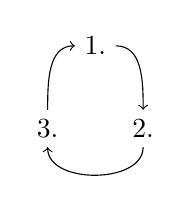
\begin{tikzpicture}[scale=.7]
\node[draw=none] (x) at (0,1) {1.};
\node[draw=none] (y) at (0.866025,-0.5) {2.};
\node[draw=none] (z) at (-0.866025,-0.5) {3.}; 
\draw[->] (x) to[in=90,out=0] (y);
\draw[->] (y) to[in=-90,out=-90] (z);
\draw[->] (z) to[in=180,out=90] (x);
\end{tikzpicture}
\end{center}
\begin{enumerate}
\item[$(1 \implies 2)$] Let $T$ be a linear transformation, 
$a,b \in \mathbb{R}$ and $\vec{v},\vec{w} \in \mathbb{R}^n$. Then
\begin{align*}
T(a\vec{v}+b\vec{w}) &= T(a\vec{v})+T(b\vec{w})\\
&= aT(\vec{v})+bT(\vec{w})
\end{align*}
Since the choice of $a,b \in \mathbb{R}$ and $\vec{v},\vec{w} \in \mathbb{R}^n$
was arbitrary this equality holds for all choices of these values.

\item[$(2 \implies 3)$] Let $T(a\vec{v}+b\vec{w})=aT(\vec{v})+bT(\vec{w})$ for all $a,b \in \mathbb{R}$ and $\vec{v},\vec{w} \in \mathbb{R}^n$. We proceed by mathematical induction on $k$.\\[10pt] 
\begin{inparaenum}
\item[\textbf{Basis Step:}] For $k=1$ let $a_1 \in \mathbb{R}$ and 
$\vec{v}_1 \in \mathbb{R}^n$. Let $\vec{w} \in \mathbb{R}^n$ be any other 
vector. Then 
\begin{align*}
T(a_1\vec{v}_1)&=T(a_1\vec{v}_1+\vec{0})\\
&=T(a_1\vec{v}_1+0\vec{w})\\
&=a_vT(\vec{v}_1)+0T(\vec{w})\\
&=a_vT(\vec{v}_1)+\vec{0}\\
&=a_vT(\vec{v}_1)
\end{align*}

Since the choice of $a_1$ and $\vec{v}_1$ were arbitrary this equality holds 
for all $a_1 \in \mathbb{R}$ and $\vec{v}_1 \in \mathbb{R}^n$.\\[10pt] 
%
\item[\textbf{Induction Hypothesis: }] Suppose 
$T(a_1\vec{v}_1+a_2\vec{v}_2+\cdots+a_k\vec{v}_k)=
a_1T(\vec{v}_1)+a_2T(\vec{v}_2)+\cdots+a_kT(\vec{v}_k)$ for all integers $k$ 
with $1 \le k \le N$. \\[10pt] 
%
\item[\textbf{Induction: }]Let $a_1, \ldots, a_N,a_{N+1} \in \mathbb{R}$ and 
$\vec{v}_1,\ldots,\vec{v}_N,\vec{v}_{N+1} \mathbb{R}^n$. Define 
$\vec{v}=a_1\vec{v}_1+\cdots+a_N\vec{v}_N$. 

Then by the induction hypothesis $T(\vec{v})=a_1T(\vec{v}_1)+\cdots+a_NT(\vec{v}_N)$. Therefore,

\begin{align*}
T(a_1\vec{v}_1+\cdots+a_N\vec{v}_N+a_{N+1}\vec{v}_{N+1})
&=T(1\vec{v}+a_{N+1}\vec{v}_{N+1})\\
&=1T(\vec{v})+a_{N+1}T(\vec{v}_{N+1})\\
&=a_1T(\vec{v}_1)+\cdots+a_NT(\vec{v}_N)+a_{N+1}T(\vec{v}_{N+1})
\end{align*}
Which proves this case by mathematical induction.
\end{inparaenum}

\item[$(3 \implies 1)$] Suppose 
$T(a_1\vec{v}_1+a_2\vec{v}_2+\cdots+a_k\vec{v}_k)=
a_1T(\vec{v}_1)+a_2T(\vec{v}_2)+\cdots+a_kT(\vec{v}_k)$ for all integers $k$ with $k \ge 1$.

Let $r\in \mathbb{R}$ and $\vec{v} \in \mathbb{R}^n$.
Then consider the $k=1$ case $a_1=r$ $\vec{v}_1=\vec{v}$. Then 
\begin{align*}
T(r\vec{v})&=T(a_1\vec{v}_1)\\
&=a_1T(\vec{v}_1)\\
&=rT(\vec{v})
\end{align*}
Therefore $T$ preserves scalar multiplication.

Let $\vec{v},\vec{w} \in \mathbb{R}^2$. Consider the $k=2$ case where we let 
$a_1=a_2=1$, $\vec{v}_1=\vec{v}$ and $\vec{v}_2=\vec{w}$. Then
\begin{align*}
T(\vec{v}+\vec{w})&=T(a_1\vec{v}_1+a_2\vec{v}_2)\\
&=a_1T(\vec{v}_1)+a_2T(\vec{v}_2)\\
&=1T(\vec{v})+1T(\vec{w})\\
&=T(\vec{v})+T(\vec{w})
\end{align*}
Thus $T$ also preserves vector addition and is therefore a 
linear transformation.
\end{enumerate}
\end{proof}

\subsubsection{Exercises} \relax
%\addcontentsline{toc}{subsubsection}{Exercises}


\subsection{The Standard Matrix of a Linear Transformation}
\index{The Standard Matrix of a Linear Transformation}

\begin{definition}
If linear transformation $T:\mathbb{R}^n \to \mathbb{R}^m$ has a matrix 
$A \in M_{m\times n}(\mathbb{R})$ such that $T(\vec{v})=A\vec{v}$ then $A$ 
is called \emph{the standard matrix} of $T$.
\end{definition}

\begin{theorem} Every linear transformation $T:\mathbb{R}^n \to \mathbb{R}^m$ 
has a standard matrix $A=[\vec{a}_1,\vec{a}_2, \ldots, \vec{a}_n]$. In fact,
$\vec{a}_k=T(\vec{e}_k)$ for each integer $k$ with $1 \le k \le n$ 
where $\{\vec{e}_1,\vec{e}_2,\ldots,\vec{e}_n\}$ are the standard basis for 
$\mathbb{R}^n$.\label{thm:standard_matrix}
\end{theorem}

\begin{proof}
It suffices to show that $T(\vec{v})=A\vec{v}$ for all 
$\vec{v} \in \mathbb{R}^n$.
Let $\vec{v} \in \mathbb{R}^n$ be an arbitrary, but fixed, vector. By 
Proposition~\ref{prop:e_k_spans_Rn} $\vec{v}$ is a linear combination of the 
standard basis. In fact, it can be written:
\[
\vec{v}=v_1\vec{e}_1+v_2\vec{e}_2+\cdots+v_n\vec{e}_n
\]

where the each $v_k$ is the $k^{\text{th}}$ coordinate of $\vec{v}$. Thus
\begin{align*}
T(\vec{v}) 
&=T(v_1\vec{e}_1+v_2\vec{e}_2+\cdots+v_n\vec{e}_n)\\
&=v_1T(\vec{e}_1)+v_2T(\vec{e}_2)+\cdots+v_nT(\vec{e}_n)\\
&=v_1\vec{a}_1+v_2\vec{a}_2+\cdots+v_n\vec{a}_n\\
&=[\vec{a}_1,\vec{a}_2,\ldots,\vec{a}_n]
\begin{bmatrix}v_1\\v_2\\\vdots\\v_n\end{bmatrix}\\
&=A\vec{v}
\end{align*}
\end{proof}

\begin{example} Let's find the standard matrix for the linear transformation
$T:\mathbb{R}^2 \to \mathbb{R}^3$ 
defined by 
$T\begin{bmatrix}v_1 \\ v_2 \end{bmatrix}=
\begin{bmatrix}v_1-3v_2\\v_2\\5v_1-3v_2\end{bmatrix}$.

Since the domain is $\mathbb{R}^2$ we use the standard basis $\{\vec{e}_1,\vec{e}_2\}$ for $\mathbb{R}^2$. 
\begin{alignat*}{9}
\vec{a}_1
&=T(\vec{e}_1) 
&= T\begin{bmatrix}1 \\ 0\end{bmatrix} &=\begin{bmatrix}1\\0\\5\end{bmatrix}
&\hspace*{1.5cm} &\vec{a}_2
&=T(\vec{e}_2) 
&= T\begin{bmatrix}0 \\ 1\end{bmatrix} 
&=\begin{bmatrix*}[C]-3\\1\\-3\end{bmatrix*}
\end{alignat*}
So $A=\begin{bmatrix*}[c]1 & -3 \\0 & 1 \\5 & -3\\\end{bmatrix*}$
We can test our work simply by multiplying:
\[
A\begin{bmatrix}v_1 \\ v_2 \end{bmatrix}
=\begin{bmatrix*}[c]1 & -3 \\0 & 1 \\5 & -3\\\end{bmatrix*}
\begin{bmatrix}v_1 \\ v_2 \end{bmatrix}
=\begin{bmatrix}
v_1-3v_2 \\ v_2 \\ 5v_1-3v_2
\end{bmatrix}
\]
\end{example}
By combining Theorem~\ref{thm:standard_matrix} and 
Proposition~\ref{prop:Av_is_linear} we can use the existence of a standard matrix to prove or disprove a particular function is linear. 
\begin{example}
For example consider $T:\mathbb{R}^4 \to \mathbb{R}$ defined by
\[
T\begin{bmatrix}v_1 \\ v_2 \\ v_3 \\ v_4 \end{bmatrix}=5v_1-3v_3+v_4
\]

$T(\vec{e}_1)=5$, $T(\vec{e}_2)=0$, $T(\vec{e}_3)=-3$ and $T(\vec{e}_4)=1$ so 
$A=\begin{bmatrix}5 & 0 & -3 & 1\end{bmatrix}$

By checking, 
\[
\begin{bmatrix}5 & 0 & -3 & 1\end{bmatrix}
\begin{bmatrix}v_1 \\ v_2 \\ v_3 \\ v_4 \end{bmatrix}
=5v_1+0v_2-3v_3+v_4=T(\vec{v})
\]
We prove that $T$ can be written as a matrix-vector product and therefore is 
a linear transformation.
\end{example}

\begin{example}
Consider the function $T:\mathbb{R}^3\to \mathbb{R}^2$ via
\[
T\begin{bmatrix}v_1 \\ v_2 \\ v_3 \end{bmatrix}
=\begin{bmatrix}3v_1-2v_2^2 \\ 3+v_2\end{bmatrix}
\]
This function is not linear but we can still make what looks like a
matrix for it:\\ 
$T(\vec{e}_1)=\begin{bmatrix}3\\3\end{bmatrix}$ 
$T(\vec{e}_2)=\begin{bmatrix}-2\\4\end{bmatrix}$ 
and $T(\vec{e}_3)=\begin{bmatrix}0\\3\end{bmatrix}$.

So wouldn't $A=\begin{bmatrix*}[C] 3 & -2 & 0 \\ 3 & 4 & 3 \end{bmatrix*}$ ??

Checking the multiplication reveals the problem,

$A\vec{v}=\begin{bmatrix}3v_1-2v_2\\3v_1+4v_2+3v_3\end{bmatrix}
\neq \begin{bmatrix}3v_1-2v_2^2 \\ 3+v_2\end{bmatrix}$

Therefore $T$ does not have a standard matrix so is not a linear 
transformation.
\end{example}
\input{Rn/Linear_Transformations_Standar_Matrix_exercises.tex}

\section{Geometry of $\mathbb{R}^n$}

Each vector $\begin{bmatrix}v_1\\v_2 \\ \vdots \\ v_n \end{bmatrix} \in \mathbb{R}^n$ can be visualized as an arrow going from the origin 
$(0,0, \ldots, 0)$ to the point $(v_1, v_2, \ldots, v_n)$.  In this case we'd call the \textbf{base point} the origin.

\begin{example}
$\begin{bmatrix}2\\5\end{bmatrix}$ can be visualized as the arrow between $(0,0)$ and $(2,5)$\\
  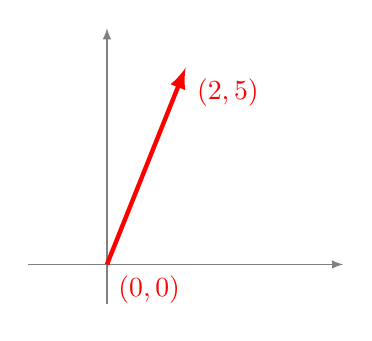
\begin{tikzpicture}[scale=.5]
    \coordinate (Origin)   at (0,0);
    \coordinate (XAxisMin) at (-2,0);
    \coordinate (XAxisMax) at (6,0);
    \coordinate (YAxisMin) at (0,-1);
    \coordinate (YAxisMax) at (0,6);
    \draw [thin, gray,-latex] (XAxisMin) -- (XAxisMax);% Draw x axis
    \draw [thin, gray,-latex] (YAxisMin) -- (YAxisMax);% Draw y axis
    \draw [ultra thick,-latex,red] (Origin) node [below right] {$(0,0)$} -- (2,5) node [below right] {$(2,5)$};
  \end{tikzpicture}
\end{example}

We can also think of any arrow from point $(a_1, a_2, \ldots, a_n)$ to point $(b_1, b_2, \ldots, b_n)$ as a vector. We've simply changed 
the \text{base point} to $(a_1, a_2, \ldots, a_n)$ instead of the origin. 

\begin{definition}
The \textbf{canonical form} of a vector from $(a_1, a_2, \ldots, a_n)$ to $(b_1, b_2, \ldots, b_n)$ is the vector 
$\begin{bmatrix}b_1-a_1 \\ b_2-a_2 \\ \vdots \\ b_n-a_n\end{bmatrix}$
\end{definition}

\begin{remark}
You can think of the canonical form of a vector is taking an arrow with the same length and direction with base point of the origin.
\end{remark}

\begin{example}
The vector from $(2,3)$ to $(3,-2)$ has canonical form $\begin{bmatrix}1\\-5\end{bmatrix}$. Below the vector is in red and the canonical form of the vector is in blue.\\
  \begin{tikzpicture}[scale=.5]
    \coordinate (Origin)   at (0,0);
    \coordinate (XAxisMin) at (-6,0);
    \coordinate (XAxisMax) at (6,0);
    \coordinate (YAxisMin) at (0,-6);
    \coordinate (YAxisMax) at (0,6);
    \draw [thin, gray,-latex] (XAxisMin) -- (XAxisMax);% Draw x axis                                                                                                   
    \draw [thin, gray,-latex] (YAxisMin) -- (YAxisMax);% Draw y axis                                                                                                   
    \draw [ultra thick,-latex,red] (2,3) node [above right] {$(2,3)$} -- (3,-2) node [above right] {$(3,-2)$};
    \draw [ultra thick,-latex,blue] (Origin) node [above right] {$(0,0)$} -- (1,-5) node [above right] {$(3,-2)$};
  \end{tikzpicture}
\end{example}

\section{SYSTEMS OF LINEAR EQUATIONS}
\index{Systems of Linear Equations}

A linear equation with variables $x_1$, $x_2$ is something of the form
$$
a_1x_1+a_2x_2=b
$$
for some constants $a_1$, $a_2$, and $b$.

\section{Gauss-Jordan Elimination}
\subsection{Solving Systems of Equations}
\subsubsection{Exercises}
\begin{exercise}
Find the solution set to the following system of equations using elementary equation operations.\\
\begin{inparaenum}[a)]
\item $\left\{ \begin{matrix} x&+&2y &=&1 \\ 2x&-&3y &= &0 \end{matrix}\right. $ \hfill
\item $\left\{ \begin{matrix} x&+&y &=&1 \\ x&+&y &= &0 \end{matrix}\right. $ \hfill
\item $\left\{ \begin{matrix} x&+&y &=&1 \\ x&-&y &= &0 \end{matrix}\right. $ \hfill {} \\
\item $\left\{ \begin{matrix} x&+&y&+&z &=&1 \\ 2x&-&3y& & &= &0 \\ & & & & z&=&1\end{matrix}\right. $ \hfill
\item $\left\{ \begin{matrix} 2x&+&3y &=&6 \\ 5x&+&2y &= &1 \end{matrix}\right. $ \hfill
\item $\left\{ \begin{matrix} x&+&y &=&1 \\ 2x&+&2y &= &2 \end{matrix}\right. $ \hfill {} \\
\end{inparaenum}
\end{exercise}


\subsection{Augmented Matrices and Row Operations}
\subsubsection{Exercises}
\input{Rn/Gauss_Augmented_exercises}

\subsection{Solutions to Homogeneous and Inhomogeneous Systems}
\subsubsection{Exercises}
\input{Rn/Gauss_Hom_Inhom_exercises}





 % CHAPTER 1

\appendix

\chapterimage{Pictures/chapter_head_2.pdf} % Chapter heading image
\chapter{Appendix}
\section{The Principle of Mathematical Induction}
\index{Induction}

\begin{theorem*}[Theorem~\ref{thm:linear_transformation_equivalences}]
Let $T:\mathbb{R}^n\to\mathbb{R}^m$ be a function. The following are equivalent:
\begin{enumerate}
\item $T$ is a linear transformation.
\item $T(a\vec{v}+b\vec{w})=aT(\vec{v})+bT(\vec{w})$ for all $a,b \in \mathbb{R}$
and $\vec{v},\vec{w} \in \mathbb{R}^n$
\item $T(a_1\vec{v}_1+a_2\vec{v}_2+\cdots+a_k\vec{v}_k)=                                                                                                                
a_1T(\vec{v}_1)+a_2T(\vec{v}_2)+\cdots+a_kT(\vec{v}_k)$
for all $a_i \in \mathbb{R}$ and $\vec{v}_i \in \mathbb{R}^n$ and $k$ a positive integer.
\end{enumerate}
\end{theorem*}


\begin{proof} ($2 \implies 3$)
\begin{inparaenum}
\item[\textbf{Basis Step:}] For $k=1$ let $a_1 \in \mathbb{R}$ and
$\vec{v}_1 \in \mathbb{R}^n$. Let $\vec{w} \in \mathbb{R}^n$ be any other
vector. Then
\begin{align*}
T(a_1\vec{v}_1)&=T(a_1\vec{v}_1+\vec{0})\\
&=T(a_1\vec{v}_1+0\vec{w})\\
&=a_1T(\vec{v}_1)+0T(\vec{w})\\
&=a_1T(\vec{v}_1)+\vec{0}\\
&=a_1T(\vec{v}_1)
\end{align*}

Since the choice of $a_1$ and $\vec{v}_1$ were arbitrary this equality holds
for all $a_1 \in \mathbb{R}$ and $\vec{v}_1 \in \mathbb{R}^n$.\\[10pt]
%                                                                                                                                                                       
\item[\textbf{Induction Hypothesis: }] Suppose \\
$T(a_1\vec{v}_1+a_2\vec{v}_2+\cdots+a_k\vec{v}_k)=                                                                                                                      
a_1T(\vec{v}_1)+a_2T(\vec{v}_2)+\cdots+a_kT(\vec{v}_k)$ for all integers $k$
with $1 \le k \le N$. \\[10pt]
%                                                                                                                                                                       
\item[\textbf{Induction: }]Let $a_1, \ldots, a_N,a_{N+1} \in \mathbb{R}$ and
$\vec{v}_1,\ldots,\vec{v}_N,\vec{v}_{N+1} \in \mathbb{R}^n$. Define
$\vec{v}=a_1\vec{v}_1+\cdots+a_N\vec{v}_N$.

Then by the induction hypothesis $T(\vec{v})=a_1T(\vec{v}_1)+\cdots+a_NT(\vec{v}_N)$. Therefore,

\begin{align*}
T(a_1\vec{v}_1+\cdots+a_N\vec{v}_N+a_{N+1}\vec{v}_{N+1})
&=T(1\vec{v}+a_{N+1}\vec{v}_{N+1})\\
&=1T(\vec{v})+a_{N+1}T(\vec{v}_{N+1})\\
&=a_1T(\vec{v}_1)+\cdots+a_NT(\vec{v}_N)+a_{N+1}T(\vec{v}_{N+1})
\end{align*}
Which proves this case by mathematical induction.
\end{inparaenum}
\end{proof}

\section{Inverse Functions}
\index{Inverse Functions}

\input{Appendix/Cardinality}






%%----------------------------------------------------------------------------------------
%	BIBLIOGRAPHY
%----------------------------------------------------------------------------------------

%\chapter*{Bibliography}
%\addcontentsline{toc}{chapter}{\textcolor{ocre}{Bibliography}}
%\section*{Books}
%\addcontentsline{toc}{section}{Books}
%\printbibliography[heading=bibempty,type=book]
%\section*{Articles}
%\addcontentsline{toc}{section}{Articles}
%\printbibliography[heading=bibempty,type=article]
\nocite{*}
\bibliographystyle{plain}
\bibliography{bibliography}
\addcontentsline{toc}{chapter}{\textcolor{ocre}{Bibliography}}
%----------------------------------------------------------------------------------------
%	INDEX
%----------------------------------------------------------------------------------------

\cleardoublepage
%\phantomsection
%\setlength{\columnsep}{0.75cm}
%\addcontentsline{toc}{chapter}{\textcolor{ocre}{Index}}
%\printindex

%----------------------------------------------------------------------------------------



\backmatter

\nocite{*}
\bibliographystyle{plain}
\bibliography{bibliography}
\addcontentsline{toc}{chapter}{\textcolor{bookcolor}{Bibliography}}

\printindex
\clearpage
\addcontentsline{toc}{chapter}{\textcolor{bookcolor}{Index}}

\end{document}
